\documentclass{article}
\usepackage{pslatex}
\usepackage{indentfirst}
\usepackage{amssymb,amsmath,amsthm,amscd,bm}
\usepackage{graphicx}


\author{Fokin Alexander\\ \texttt{ru.elric[at]gmail.com} }
\title{Implementing Real-time Ray Tracing Engine for use in Virtual Reality System}

\begin{document}

\pagestyle{empty}
\maketitle
\thispagestyle{empty}
\cleardoublepage
\tableofcontents
\cleardoublepage
\pagestyle{headings}
\setcounter{page}{3}

\section*{Abstract}
During the last several decades of research in the field of computer graphics, one of the main goals was to find a way to generate realistic images at interactive frame rates. As it is of today, almost all real-time rendering systems rely on the technology of triangle rasterization. Despite the fact that this technology was constantly being improved during the last several decades, it still has a lot of limitations. Even with today's hi-end hardware and all the advance in programming interfaces, implementation of complex effects, including shadows, reflections, or refractions, still require a lot of difficult programming and produces only an approximation of these effects, which fail in some cases.

An alternative to rasterization, which doesn't have these limitations, and is known for its flexibility and high degree of achievable realism, is ray tracing. With ray tracing one gets all the above-mentioned effect in a physically correct way, and almost for free, i.e. without any complicated programming required. The problem with ray tracing is in its high computational cost, and that's why for a long time it was used only for offline rendering. However, with the huge advance in performance of commodity personal computers, a lot of research has been done in the field of interactive ray tracing. With the use of a newly developed techniques, it has been shown that ray tracing of complex dynamic environments is possible on interactive frame rates even on commodity personal computers. Ray tracing still cannot compete with rasterization in terms of rendering speed, but in terms of realism it is definitely better.

In this work we present a short overview of different optimization techniques used in modern interactive ray tracing engines. Then we discuss the design principles and optimizations used in SMART \footnote[1]{SMART stands for SMART Minimalistic Arx Ray Tracer}, our real-time ray tracing system. In the end we describe some of the details of using SMART with CAVE virtual reality system.

\newpage
\section{Introduction}
Recently, with the huge advance in performance of processors, interactive ray tracing on commodity personal computers became possible. Interactivity implies dynamic scenes, which change unpredictably, depending on the user input, and therefore it's impossible to apply sophisticated preprocessing algorithms used in offline rendering to speed up the ray tracing of such scenes. Instead, fast preprocessing algorithms were proposed for building acceleration structures of decent quality \cite{wald04}. With the use of these techniques, along with optimizations for modern architectures, it became possible to render dynamic scenes at almost real-time speeds on a single PC.

The obvious question is where real-time ray tracing rendering can be used today. It is still too slow for games, and in most games physically correct rendering is not the necessity - approximations provided by the use of modern rasterization hardware in most cases produce decent results. Maybe in a few years, with the increase of computational power of commodity PCs, the situation would change. Optimized interactive ray tracing can also aid in the fields where ray tracing was traditionally the only approach, such as industrial rendering. But anyway, in such areas real-time rendering again is not the necessity - of course it can be used for pre-rendering, but final images are almost always produced with offline bidirectional monte carlo ray tracing renderer, such as Mental Ray \cite{mentalray}. One of the fields which today can benefit from the utilization of real-time ray tracing is virtual reality. In VR systems realism was always of high importance, and such systems are almost always ahead of the commodity PCs in terms of computational power, therefore they can greatly benefit from usage of modern real-time ray tracing rendering techniques.

Originally ray tracing computations were performed on CPU only, and it was impossible to utilize the tremendous computational power of graphical accelerators to speed it up, since they were using a fixed rendering pipeline, applicable for rasterization only. But with the introduction of programmable rendering pipeline, and its further development, it became possible to move some of the ray tracing computations to GPU. In this work we will first provide an overview of existing CPU-based interactive ray tracing solutions and the differences of CPU-based and GPU-based approaches. Then we will describe our CPU-based interactive ray tracing system.


\newpage
\section{Real-time Ray Tracing on CPU}

\subsection{Overview of Existing Solutions}
As it is of now, it is still impossible to render complex ray traced scenes in real-time on a single CPU, but we are sure that in a few years it will become real. Today the most impressive attempts of implementing an application based on real-time ray tracing engine are Q4RT \cite{q4rt}, and recently presented at Intel's 2008 research day QWRT \cite{qwrt} projects - ray traced Quake 4 and Quake Wars respectively. Yet even these demonstrations, implemented on top of the state-of-the-art coherent ray tracer, are unable to run in real-time on a single modern CPU. The best frame rates achieved by QWRT were 15-20 frames per second at 1280x720 on a Caneland system that has four Tigerton quad-cores in it (total 16 cores), clocked at 2.93 GHz.

Supposedly the most well-known real-time ray tracing engine today is OpenRT \cite{openrt}. It features not only standard ray-tracing of dynamic scenes, but also global illumination and, to some extent, caustic effects. Such projects as Q3RT \cite{q3rt} and Q4RT \cite{q4rt} were built on top of that engine. Developers of OpenRT took the brute force approach instead of using sophisticated approximations like Render Cache \cite{walter99}, which often result in artifacts and eat up a lot of processing power which could have been spent on shooting rays. 

Another well-known project is Aurana \cite{aurana}. The project is relatively young, and it doesn't offer all the functionality that OpenRT has, but it is open source, and therefore can be used for rendering in any GPL project. In contrast to OpenRT, authors of Aurana decided to trade flexibility of the engine for performance, and the result is quite impressive - this engine outperforms the above-mentioned systems, offering real-time rendering speeds even on single-CPU systems. Even though Aurana uses fixed rendering pipeline, it is still quite flexible, since this pipeline can be easily tweaked for the needs of any particular application.

\subsection{Commonly Used Optimizations}

\subsubsection{General Design}
As denoted above, modern real-time ray tracing engines mostly use brute force solutions, which simplify the overall design, as well as guarantee no rendering artifacts. Since the biggest part of processing power is spent on tracing acceleration structures and testing for ray-object intersections, these routines are carefully optimized. Almost all of today's real-time ray tracing engines work only with triangles. This speeds up the rendering, because of less branches needed to be taken, and doesn't really impact the capabilities of the engine, since any object can be represented as a polygonal model.

\subsubsection{Paying Attention to Architectural Features}
Ray tracing has proved to scale almost perfectly, therefore it greatly benefits from the presence of multiple cores. On multicore systems rays are traced in several threads, and with a careful addressing of caching issues, ray tracing scales almost linearly with the increase of the number of cores. Carefully optimized ray tracers utilize all of the computational power of the CPU, and that's why they do not benefit from the support of Hyper-Threading or similar technologies, which were designed to prevent processor stalls.

Modern ray tracers also get a major speedup from the use of SSE (or AltiVec) technology. Careful use of SSE allows for simultaneous tracing of four rays instead of one, which results in up to 200\% speedup. But the usage of SSE also greatly increases the complexity of ray tracer and gives rise to a lot of problems, such as different rays in packet taking different routes when tracing acceleration structure. All these problems have long been known, and a lot of research has been done in this field.

One of the really important issues to be addressed when implementing a real-time ray tracer is memory layout optimization, as well as careful precaching. Normally, a cache miss results in a processor stall for over one hundred cycles, and therefore the number of such stalls should be minimized. Of course, modern processors include sophisticated precaching algorithms, but using manual precaching together with carefully designed memory layout gives much better results. Issues to address when dealing with memory layout design include alignment to cache line, for cache miss not to result in two cache entries to be renewed, and exploiting the data locality. For example, it is a good idea to store the data used for ray-triangle intersection tests and the data used during shading separately, because the latter isn't needed for intersection testing, as well as the first one isn't needed for shading. The general rule is as follows: optimize data layout in way that prefetch or cache update operations load only the data that will be actually used in calculations. Also it is important to issue prefetch instructions as soon as possible.

Another way to improve cache performance of the algorithm is to exploit coherency. The simplest way to do it is to trace rays not line-by-line, but in tiles of fixed size. Rays that are close to each other are likely to go through the same nodes of acceleration structure, and hit the same primitives, therefore increasing the locality of data accesses.

Also an important issue arises when using multicore and multiprocessor systems. In such systems, writing to the memory shared between cores should be avoided, because such write performed on one core invalidates the whole cache line on other cores, therefore resulting in processor stalls.


\subsubsection{Ray-Triangle Intersection}
While the above-described optimizations rely on architectural features, algorithmic optimizations are also of great importance. The first thing to optimize is ray-triangle intersection function. In fact, there exist a lot of different algorithms, but most of them follow a single general pattern. This pattern uses barycentric coordinates coupled with projection method and a lot of precalculation to speed up the intersection test \cite{wald04, badouel92}.

\subsubsection{Acceleration Structure}
But the most important issue to address when talking about optimizing ray tracing is, of course, the acceleration spatial subdivision structure used. There are many approaches to this, which include regular grids and octtrees \cite{dmitriev00}, BSP trees and bounding volume hierarchies. It has been shown, that axis-aligned BSP trees usually perform at least comparable to other techniques \cite{havran01}. The only problem is that acceleration structures building algorithms are time-consuming, and therefore not always applicable for real-time rendering of dynamic scenes. For dynamic scenes, the best results were shown by bounding volume hierarchies, which allow for dynamic restructuring in linear time \cite{yoon07}.

Along with the type of the acceleration structure used, the building algorithm is also of great importance. In has been shown that by simply using different algorithms for BSP tree construction one can archive a 2x speedup \cite{wald04}. It seems that the most widely used approach is the one based on surface area heuristic. For building axis-aligned BSP trees with this approach there has been developed an algorithm with $O(N log N)$ complexity \cite{wald06}.


\newpage
\section{Real-time Ray Tracing on GPU}

\subsection{Overview of Existing Solutions}
Given the computational power of modern graphical accelerators used for rasterization, it is really tempting to try to use them for ray tracing - GPUs are highly parallel, and ray tracing has shown to be scaling almost linearly with the increase in number of processing units. The field of GPU ray tracing is relatively young, with a little research done. This is mostly due to the fact that GPUs which can be used for general purpose computations have appeared only several years ago. Before that there was some research done on exploiting GPUs for ray-tracing, but the results weren't that impressive, mostly due to the high overhead of CPU-GPU communications and the limitations of the GPU architecture \cite{purcell02}. With today's modern GPUs and general purpose GPU programming interfaces like NVIDIA CUDA \cite{cuda} it became possible to move almost all of ray tracing computations to GPU, therefore allowing for high performance. The latest example of such approach was shown by NVIDIA at NVISION 2008, where they have demonstrated a fully interactive GPU-based ray tracer. Authors have used four next-generation Quadro GPUs in an NVIDIA Quadro Plex 2100 D4 Visual Computing System to render a complex, two-million polygon, anti-aliased scene at up to 30 frames per second at a resolution of 1920x1080 \cite{luebke08}.

Because the field of GPU ray tracing is relatively young, currently there are no general-purpose GPU ray tracing solutions available. All the systems presented up to now are technical demos, which lack a well-defined programming interface and flexibility of the above-mentioned CPU raytracers like OpenRT or Aurana.

\subsection{Commonly Used Optimizations}

\subsubsection{General Design}
Generally, almost everything written above about ray-tracing on CPU also applies to GPU. On GPU BSP trees are also used, and it is even possible to construct these trees solely on GPU \cite{zhou08}. The only significant difference is architectural one.

\subsubsection{Paying Attention to Architectural Features}
GPU architecture is highly parallel, and benefits most from several concurrent threads executing the same sequence of instructions. That's why algorithms with complicated logic, i.e. with a lot of branch instructions, aren't always preferable. Also GPU doesn't support recursion, and therefore to use any of CPU-side algorithm a non-recursive equivalent must first be derived. Although it doesn't seem a major limitation at a first glance, it is one when taking recursive nature of ray tracing into account. In current implementations by NVIDIA this problem is solved by creating a local stack of fixed size and rewriting an algorithm to use it \cite{luebke08}.

\subsubsection{Combining CPU and GPU}
Taking Moore's law into account, in a few years it will be possible to run the above-mentioned ray tracing applications on decent frame rates on commodity PCs. But considering the fact that most PCs come bundled with a decent GPU, it is also possible to use CPU and GPU simultaneously, therefore allowing for a significant speedup of current CPU-based ray tracers. The problem of such approach is that CPU and GPU architectures are different, and therefore require different algorithms and data structures for archiving optimal performance.

Another major problem is the small amount of memory available on GPUs compared to what we have for CPUs. While it is theoretically possible to store some of the structures used by GPU ray tracer in RAM, and moving it to GPU memory only when they are needed, it is not practical, mostly because of high latencies of such operation and overall complication of the algorithm. Therefore, the application of modern GPUs for ray tracing of complex scenes is rather limited, but they still can be used to aid CPU-based ray tracing.

Even though it's possible to implement a task-driven rendering core that would dispatch rendering tasks both to CPU and GPU, the developers of such a system will have to solve these problems, and as it is of now, no such system has been created.


\newpage
\section{Our Implementation}
Taking all the above mentioned factors into account, we've decided to focus on CPU-based ray tracing for our implementation. Some of implementation details of our approach are described below.

\subsection{General Design}
The main design rule we followed during the development of SMART system was never to sacrifice the flexibility of the engine, unless it's sacrificed for performance. The main features of our system are:

\begin{enumerate}
\item Triangle geometry. SMART works with triangles only. This restriction increases the performance of ray tracer, while not imposing a major penalty on the flexibility -- anyway, almost all of the real-world models use triangle representation.
\item Axis-aligned BSP tree as acceleration structure for geometry. BSP trees have shown to perform at least not worse than any other acceleration structures, while allowing for a very simple, and therefore really fast traversal implementation. Another benefit of BSP trees is that the implementation of ray packet traversal for them is rather straightforward, which is not generally true for other acceleration structures.
\item $O(N\log{N})$ BSP tree building, as described in \cite{wald06}. We use fast BSP tree building algorithm based on Surface Area Heuristic, which produces high quality BSP trees, while offering a complexity of $O(N\log{N})$, which is a theoretical lower bound for {\it any} BSP tree building algorithm.
\item Two-level acceleration structure. SMART operates on immutable geometry units - models. Each model consists of several triangles, and cannot be changed once compiled. This means that for each model we have to build a BSP tree only once -- at the time of model construction, and then it's we can reuse it during rendering. To allow for dynamic scenes, compiled models are inserted into a top-level global BSP tree, which is rebuilt every frame. Models, which are generated anew each frame could also be used with this approach, but they will require another BSP tree building algorithm, which will produce BSP trees of worse quality, but faster.
\item Multithreaded rendering. SMART automatically determines the number of available cores and performs rendering in the corresponding number of threads. Load balancing is done automatically, so that when double buffering is used, rendering threads doesn't stall between frames, therefore utilizing all the available computational power.
\item Carefully optimized triangle intersection and BSP tree traversal routines. Ray tracer spends most of the rendering time in these routines, therefore they must be extremely optimized. We use the method described by Ingo Wald in his Ph.D. thesis \cite{wald04}, with some slight modifications to pay attention to numerical stability issues.
\item Fully programmable shading. SMART uses shaders written in C++, therefore allowing for shaders of any complexity. It is possible to shoot additional rays from a shader, as well as perform visibility checks, which makes even the implementation of such complicated effects as BRDFs rather straightforward (but of course, implementing BRDFs will move us back to the field of offline rendering). While fully programmable shading offers a lot of benefits, it also degrades the performance in case only one shader type is needed. SMART was designed in way so that in such cases it would be possible to replace the programmable shading functionality with a fixed one just by passing a fixed shader as a C++ template parameter to the core, without the need to reimplement any of the core functionality, as it is in OpenRT.
\item Partial compatibility with OpenRT programming interface \cite{dietrich03}. Even though SMART core uses its own interface, adapter which supports a part of OpenRT functionality was written. OpenRTS shading interface is not yet supported, but implementing it will also be straightforward. Even now, with a lot of OpenRT commands unsupported, poring OpenGL programs to SMART is fast is simple.
\end{enumerate}

\subsubsection{Overall Data Structure}
As it was mentioned above, in a ray tracer it is better to separate storage for triangle and shading data, since the first one is used during intersection tests, and the second one - during shading. Moreover, separating shading and triangle data makes it possible to use the same set of triangles with several different sets of shaders, therefore allowing for "reshading" of existing models without actual copying of underlying triangle data or rebuilding of BSP tree. The same goes for the whole scene, because the scene can be thought of as a special kind of model, which has models instead of triangles as its elements. That gives rise to the following overall structure:

\begin{center}
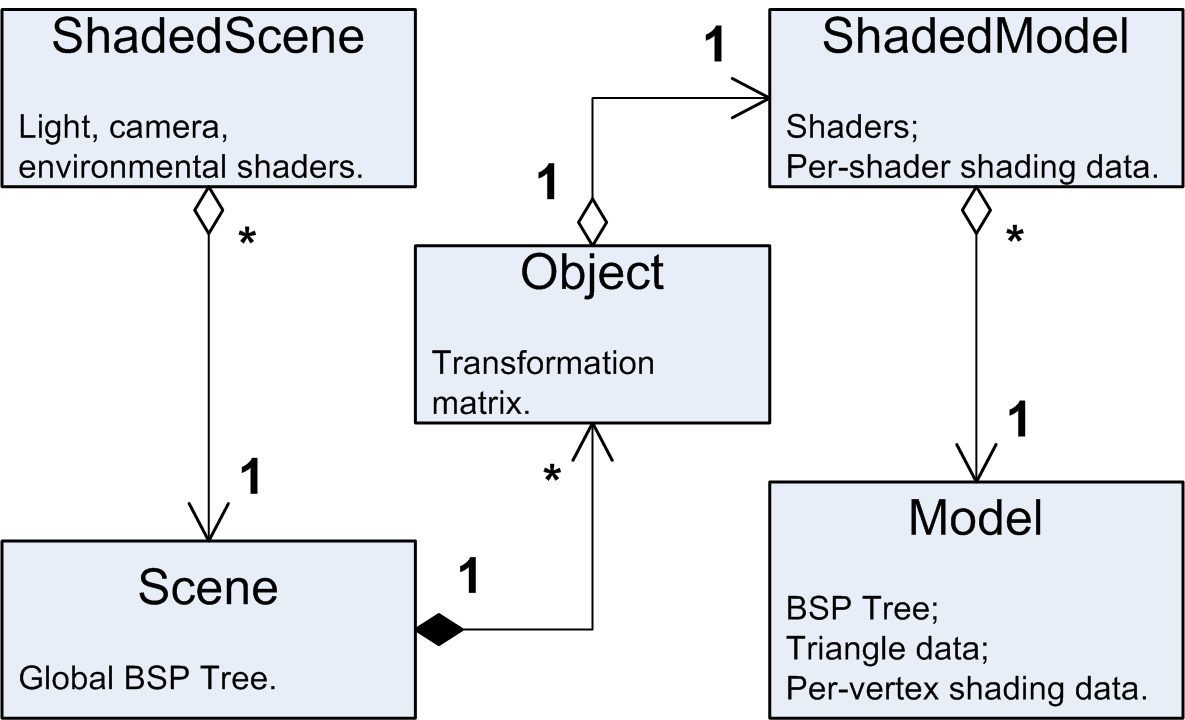
\includegraphics[width=80mm]{Overall.png}
\end{center}

Double-buffering rendering approach implies that while one scene is being rendered, the other one is being constructed. This means that in the same moment there exist several scene instances. Our approach further develops this idea by allowing to work on multiple scenes simultaneously and queue them for rendering in a bunch.

\subsubsection{Rendering}
Rendering subsystem is separated from the geometry processing core, and its design allows for rendering workers to be not only CPU threads, but also, for example, remote clients connected over ethernet network. Even though the parallelization over several PCs is not yet implemented, the possibility that it may be needed was taken into account when designing the overall structure of the system, and therefore adding such functionality won't require a complete rewrite. Instead, it will be sufficient just to reimplement a rendering worker interface for the case when rendering is done on a remote machine.

As it is of now, rendering is done in several threads, with the number of threads equal the number of cores of the processor used. Before rendering, frame buffer is divided into tiles, and then these tiles are dispatched to rendering threads on demand. This automatically provides a decent load balancing, as well as increases the locality of data accesses during rendering.


\subsection{Implementation Details}
The performance of SMART rendering core mostly relies on several small routines, such as ray-triangle intersection, or BSP tree traversal. One of the principles used during SMART development was to apply algorithmic optimizations first, and only when further tweaking of the algorithm gives no significant results, revert to low-level optimizations. 

Here we are going to describe the algorithmic optimizations used in SMART.

\subsubsection{Ray-Triangle Intersection}
We are using an approach developed by Ingo Wald \cite{wald04}, which is a based on barycentric coordinates method. First, a signed distance along the ray to the triangle plane is computed. If we denote ray origin as $O$, direction vector as $D$, and three triangle vertices as $A$, $B$, and $C$, then this distance can be calculated as follows:

$$t_{plane} = - \frac{(O - A) \cdot N}{D \cdot N}\text{,}$$

where $N$ denotes a normal: $N = (B - A) \times (C - A)$. The calculated distance is then tested for whether it lies in the interval where intersections are searched. If the test has been passed, then one has to check whether the ray actually intersects the triangle. Actual intersection point is computed as $H = O + t_{plane} D$, and is tested using barycentryc coordinates method. This can be done by solving the equation $H = \alpha A + \beta B + \gamma C$, where $\alpha$, $\beta$ and $\gamma$ are barycentric coordinates of $H$, and therefore $\alpha + \beta + \gamma = 1$ and $0 \le \alpha \le 1$, $0 \le \beta \le 1$ and $0 \le \gamma \le 1$. Note that it is sufficient to check whether $\beta \ge 0$, $\gamma \ge 0$ and $\beta + \gamma \le 1$.

The equation mentioned above is solved using projection method. Since the projection to any plane of $H$ and triangle vertices does not change the barycentric coordinates, these points can be projected to any of the coordinate planes. For numerical stability purposes the plane with the maximal projected triangle area is chosen. For example, projection on the XY plane yields:

$$ H' = \alpha A' + \beta B' + \gamma C'\text{.}$$

Substituting $\alpha = 1 - \beta + \gamma$, we get:

$$\beta (B' - A') + \gamma (C' - A') = H' - A'\text{,}$$

which is a linear system and can be easily solved. The major optimization to projection method is to precalculate as much as possible and store precalculated values in acceleration structure. In our implementation we precompute the splitting dimension, triangle normal, and coefficients for fast barycentric coordinate evaluation. We store these values in acceleration structure separately from the triangle vertex data, since for intersection testing only this acceleration structure is needed.

\subsubsection{Triangle-Box Intersection}
Another important intersection check is as check for intersection between axis-aligned bounding box and a triangle. It is used in construction of axis-aligned BSP trees and bounding volumes hierarchies. Even though an approximation can be used, it is not preferable, because it dramatically affects the quality of the resulting spatial subdivision structure, and therefore has a big impact on the rendering speed. The method we use is based on Separating Axis Theorem \cite{eberly01}. The Separating Axis Theorem tells us that, given two convex shapes, if we can find an axis along which the projection of the two shapes does not overlap, then the shapes don't overlap. In 2D, each of these potential separating axes is perpendicular to one of the edges of each shape. Separating Axis Theorem can also be extended to 3D for convex polyhedra. In three-dimensional case the set of potential separating axes consists of normal vectors to the faces of the polyhedra, and vectors generated by a cross product of two edges, one from each polyhedra.

Therefore, to check whether the triangle intersects the bounding box, the following checks are necessary:

\begin{enumerate}
\item Check for intersection of axis-aligned bounding box with the bounding box of the triangle.
\item Check for intersection in projection to triangle normal.
\item Check for intersections in projections to coordinate plane projected triangle edge normals. There are three triangle edges, three different coordinate planes, therefore we get $3 \times 3 = 9$ checks.
\end{enumerate}

This check can also benefit greatly from the usage of SSE. Axis-aligned bounding box intersection check can be implemented using SSE compare and sign extraction operations, and the most resource consuming last nine checks can be performed in three parallel groups.


\subsubsection{BSP Tree Traversal}
Since for each ray several BSP tree nodes are traversed, the traversal routine must be extremely fast. The algorithm for BSP tree traversal is rather simple: during traversal we maintain a {\it current ray segment} $[ t_{min}, t_{max} ]$, which is the parameter interval of the ray that actually intersects the current voxel. Initially this segment is initialized to $[ \epsilon, \infty ]$, and is updated incrementally during traversal. On each traversal step we calculate a distance along the ray to the splitting plane of the node:

$$d = \frac{SplitCoord - O_{splitDim}}{D_{splitDim}}\text{,}$$

where $O$ denotes the origin of the ray, $D$ -- its direction, $splitDim$ -- a splitting dimension of a node, i.e. x, y, or z, and $SplitCoord$ -- coordinate of the splitting plane. If ray segment lies completely to one side of the splitting plane, we can skip traversal of one of the subtrees and immediately proceed to the corresponding child voxel. If neither of the sides can be skipped, we traverse them in turn - the first one with segment $[ t_{min}, d ]$, and the second one with the segment $[ d, t_{max} ]$. If during traversal a valid hit point was found, a ray is terminated, and the hit point is returned. This early ray termination greatly enhances the performance of ray tracing.

While the algorithm described above implies a recursive implementation, it is better to avoid recursion in this routine. In our implementation we use a stack of nodes to be traversed, and traversal is done in a cycle. A transition from recursive to stack-based implementation gave us a speedup of over 40\%.


\subsubsection{Incorporation with the CAVELib Library}
Since we are using CAVE virtual reality system, we are forced to use CAVELib as a hardware abstraction library \cite{cavelib}. CAVELib works with OpenGL by providing custom projection and modelview matrices to user-supplied display function. Our CAVELib adapter first estimates the camera parameters based on the matrices provided by CAVELib, and then runs the ray tracer. Rendering is done into a texture, which is then passed to OpenGL and rendered as a single quad in the final pass. Camera parameter estimation is done by inversion of the product of projection and modelview matrices. Actually, this product specifies a perspective transformation from view frustum to normalized device coordinates, i.e. into cube with center at $(0, 0, 0)$ and with a side of $2$. Therefore, the inversion of this matrix performs the inverse transform, and by multiplying the coordinates of vertices of normalized device coordinates cube by it, we can calculate the actual world coordinates of the view frustum to pass them to the ray tracing engine.

\newpage
\section{Results}
Below is one of the screenshots of an application written using our ray-tracing engine.
\begin{center}
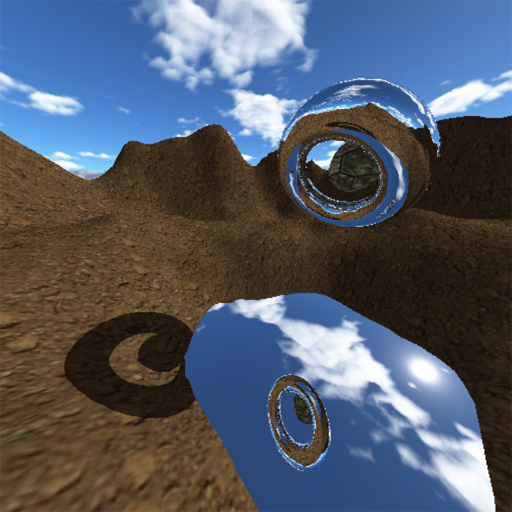
\includegraphics[width=80mm]{Screenshot.png}
\end{center}
This application runs at 10 frames per second at a resolution of 256x256 pixels on a Core 2 Duo processor clocked at 2 GHz. While this performance can be considered rather poor compared to what can be achieved with modern highly optimized ray-tracing engines such as Aurana, one should remember that SMART system is still being developed and it doesn't make use of SSE coherent ray tracing.

Our tests have shown that, just as expected for a ray tracing engine, performance of SMART scales logarithmically with the increase in the number of triangles in a scene, and linearly with the increase of a screen resolution. At a resolution of 128x128 we are getting high fps even on scenes with complex geometry and shading. We have also performed some tests at a resolution of 512x512, but on a rather simple scenes -- currently SMART cannot render complex scenes on such resolution with decent frame rates. 

\newpage
\section{Conclusion and Future Work}
In this work we have presented an overview of existing solutions in the field of interactive ray tracing. We have also developed our own real-time ray tracing system -- a SMART rendering engine, which is capable of rendering simple scenes on interactive frame rates with a decent screen resolution.

SMART system is still in development, and it presents a lot of material for optimization. First of all, we are going to implement SSE coherent ray tracing, and examine the change in performance. Then, the Multi-Level Ray Tracing approach \cite{reshetov05} can be adopted to speed up ray tracing even more.

Another thing that needs further improvement is OpenRT compatibility. Compatibility with OpenRTS shading language is also desired, but is not necessary -- mostly because of its limitations. Instead, we are currently working on a concept of a shading interface that would allow to use programmable shaders in a context of coherent ray tracer.


\newpage
\begin{thebibliography}{1}

\bibitem{wald04}
Ingo Wald: Realtime Ray Tracing and Interactive Global Illumination. PhD thesis, 2004.

\bibitem{wald06}
Ingo Wald, Vlastimil Havran: On building fast kd-trees for ray tracing, and on doing that in $O(N\log{N})$. Proceedings of the 2006 IEEE Symposium on Interactive Ray Tracing, 2006, pages 61-69.

\bibitem{purcell02}
Timothy J. Purcell, Ian Buck, William R. Mark, Pat Hanrahan: Ray Tracing on Programmable Graphics Hardware. ACM Transactions on Graphics 21, 2002, pages 703-712.

\bibitem{luebke08}
David Luebke, Steven Parker: Interactive Ray Tracing with CUDA. Presented at NVISION 2008.

\bibitem{walter99}
Bruce Walter, George Drettakis, Steven Parker: Interactive Rendering Using the Render Cache, in Rendering Techniques, 1999.

\bibitem{badouel92}
Didier Badouel: An Efficient Ray Polygon Intersection. In Graphics Gems III, 1992.

\bibitem{dmitriev00}
Kirill A. Dmitriev: Efficiency Issues on Ray Tracing Machine, 2000.

\bibitem{havran01}
Vlastimil Havran: Heuristic Ray Shooting Algorithms. PhD thesis, 2001.

\bibitem{eberly01}
David Eberly: Intersection of Convex Objects: The Method of Separating Axes. 2001.

\bibitem{zhou08}
Kun Zhou, Qiming Hou, Rui Wang, Baining Guo: Real-Time KD-Tree Construction on Graphics Hardware. 2008.

\bibitem{yoon07}
Sung-Eui Yoon, Sean Curtis, Dinesh Manocha: Ray Tracing Dynamic Scenes using Selective Restructuring. Eurographics Symposium on Rendering, 2007.

\bibitem{dietrich03}
Andreas Dietrich, Ingo Wald, Carsten Benthin, Philipp Slusallek: The OpenRT Application Programming Interface. OpenSG Symposium, 2003.

\bibitem{reshetov05}
Alexander Reshetov, Alexei Soupikov, Jim Hurley: Multi-Level Ray Tracing Algorithm. 2005.

\bibitem{openrt}
The OpenRT Real-Time Ray-Tracing Project. \\
http://www.openrt.de/

\bibitem{aurana}
Aurana realtime ray tracing. \\
http://igad.nhtv.nl/~bikker/

\bibitem{q3rt}
Quake 3: Ray Traced. \\
http://www.q3rt.de/

\bibitem{q4rt}
Quake 4: Ray Traced. \\
http://www.q4rt.de/

\bibitem{qwrt}
Quake Wars: Ray Traced. \\
http://www.qwrt.de/

\bibitem{cuda}
NVIDIA CUDA. \\
http://www.nvidia.com/cuda

\bibitem{mentalray}
Mental Images Mental Ray. \\
http://www.mentalimages.com/products/mental-ray.html

\bibitem{cavelib}
CAVELib Library. \\
http://www.mechdyne.com/integratedSolutions/software/products/CAVELib/CAVELib.htm

\end{thebibliography}


\end{document}




















